%!TEX program = xelatex
\documentclass[times,namecite]{goose-article}

\title{%
  GooseMaterial/Metal/LinearStrain/ElastoViscoPlasticHardening
}
% Former GooseFEM mat3202

\author{T.W.J.~de~Geus}

\contact{%
  $^*$Contact: %
  \href{mailto:tom@geus.me}{tom@geus.me} %
  \hspace{1mm}--\hspace{1mm} %
  \href{http://www.geus.me}{www.geus.me}%
  \hspace{1mm}--\hspace{1mm} %
  \href{https://github.com/tdegeus/GooseMaterial}{https://github.com/tdegeus/GooseMaterial}%
}

\hypersetup{pdfauthor={T.W.J. de Geus}}

\header{%
  \href{https://github.com/tdegeus/GooseMaterial}{GooseMaterial/Metal/LinearStrain/ElastoViscoPlasticHardening} -- \href{http://www.geus.me}{T.W.J.\ de Geus}%
}

\newcommand\leftstar[1]{\hspace*{-.3em}~^\star\!#1}

\begin{document}

\maketitle

\begin{abstract}
History dependent elasto-visco-plastic material. The elasticity is governed by a linear relationship between the Cauchy stress $\bm{\sigma}$ and the elastic strain $\bm{\varepsilon}_\mathrm{e}$. The material deforms elastically up to a certain yield stress (which hardens due to plasticity through a power-law). Thereafter the material deforms through a combination of elasticity and plasticity. The elastic strain depends on the strain $\bm{\varepsilon}$ (which is the symmetric part of the displacement gradient), and the history.

The model is implemented in 3-D, hence it can directly be used for either 3-D or 2-D plane strain problems.
\end{abstract}

\keywords{visco-plasticity; linear elasticity}

\setcounter{tocdepth}{2}
\tableofcontents

\vfill\newpage
\section{Constitutive model}

The model consists of the following ingredients \citep[][Chapter 11]{DeSouzaNeto2008}. To start it might be a good idea to study the one-dimensional equivalent, for completeness listed in Appendix~\ref{sec:1D}.
%
\begin{enumerate}[(i)]
%
\item The strain, $\bm{\varepsilon}$, is additively split in an elastic part, $\bm{\varepsilon}_\mathrm{e}$, and a plastic plastic, $\bm{\varepsilon}_\mathrm{p}$. I.e.
\begin{equation}
  \bm{\varepsilon} = \bm{\varepsilon}_\mathrm{e} + \bm{\varepsilon}_\mathrm{p}
\end{equation}
%
\item The stress, $\bm{\sigma}$, is set by to the elastic strain, $\bm{\varepsilon}_\mathrm{e}$, through the following linear relation:
\begin{equation}\label{eq:model:stress-elas}
  \bm{\sigma} = \mathbb{C}_\mathrm{e} : \bm{\varepsilon}_\mathrm{e}
\end{equation}
wherein $\mathbb{C}_\mathrm{e}$ is the elastic stiffness, which reads:
\begin{align}\label{eq:model:elas}
  \mathbb{C}_\mathrm{e}
  &= K \bm{I} \otimes \bm{I} + 2 G (  \mathbb{I}_\mathrm{s} - \tfrac{1}{3} \bm{I} \otimes \bm{I} )
  \\
  &= K \bm{I} \otimes \bm{I} + 2 G \, \mathbb{I}_\mathrm{d}
\end{align}
with $K$ and $G$ the bulk and shear modulus respectively. See Appendix~\ref{sec:nomenclature} for nomenclature.
%
\item The elastic domain is bounded by the following yield function
\begin{equation}
  \Phi( \bm{\sigma} , \varepsilon_\mathrm{p} )
  =
  \sigma_\mathrm{eq} - \sigma_\mathrm{y} (\varepsilon_\mathrm{p}) \leq 0
\end{equation}
where $\sigma_\mathrm{eq}$ the equivalent stress (see Appendix~\ref{sec:ap:stress}), and $\sigma_\mathrm{y}$ the yield stress which is a non-linear function of the equivalent plastic strain $\varepsilon_\mathrm{p}$. The implementation is based on power-law hardening:
\begin{equation}
  \sigma_\mathrm{y} ( \varepsilon_\mathrm{p} ) = \sigma_\mathrm{y0} + H \varepsilon_\mathrm{p}^m
\end{equation}
where $\sigma_\mathrm{y0}$ is the initial yield stress, $H$ is the hardening modulus, and $m$ is the hardening exponent.
%
\item Plasticity is governed by Norton's flow rule:
\begin{equation}\label{eq:model:epdot}
  \dot{\bm{\varepsilon}}_\mathrm{p}
  = \dot{\gamma} \, \frac{\partial \Phi}{\partial \bm{\sigma}}
  = \dot{\gamma} \, \frac{3}{2} \frac{\bm{\sigma}_\mathrm{d}}{\sigma_\mathrm{eq}}
  = \dot{\gamma} \, \bm{N}
\end{equation}
wherein $\dot{\bm{\varepsilon}}_\mathrm{p}$ is the plastic strain rate. The ratio of the stress deviator, $\bm{\sigma}_\mathrm{d}$, and it's equivalent value, $\sigma_\mathrm{eq}$, determines the direction of plastic flow (the symbol $\bm{N}$ is used to emphasize that only determines a direction, not an amplitude). The evolution of the plastic multiplier, $\dot{\gamma}$, is finally defined as follows:
\begin{equation}\label{eq:model:gammadot}
  \frac{ \dot{\gamma} }{ \dot{\gamma}_0 }
  =
  \left( \frac{\sigma_\mathrm{eq}}{\sigma_\mathrm{y}} \right)^{1/n} - 1
\end{equation}
wherein $\dot{\gamma}_0$ and the exponent $n$ are material parameters (in addition of course to the initial yield stress $\sigma_\mathrm{y0}$, the hardening modulus $H$, and the hardening exponent $m$, contained in the yield stress $\sigma_\mathrm{y}$). Note that when $\Phi \leq 0$ then $\dot{\gamma} = 0$.

Following the definition in \eqref{eq:model:epdot}, the equivalent plastic strain can be simply defined as follows:
\begin{equation}
  \varepsilon_\mathrm{p} = \int_0^t \dot{\gamma} \; \mathrm{d}\tau
\end{equation}
which corresponds to
\begin{equation}
  \dot{\varepsilon}_\mathrm{p} = \dot{\gamma}
\end{equation}
%
\end{enumerate}

\vfill\newpage
\section{Numerical implementation: implicit}

For the numerical implementation, first of all a numerical time integration scheme has to be selected. Here, an implicit time discretization is used, which has the favorable property of being unconditionally stable. To this end, the commonly used return-map algorithm is used. An increment in strain is first assumed fully elastic (elastic predictor). Then, if needed, a return-map is utilized to return to a physically admissible state (plastic corrector). The benefit of this scheme as that (i) the evolution of the plasticity (the state variable) can be determined by solving a single, albeit non-linear, equation; and that (ii) the linearization to obtain the consistent tangent operator is relatively straightforward.

\subsection{Elastic predictor}

Given an increment in strain
\begin{equation}
  \bm{\varepsilon}_\Delta = \bm{\varepsilon}^{(t + \Delta t)} - \bm{\varepsilon}^{(t)}
  \label{eq:strain-increment}
\end{equation}
and the state variables, the \emph{elastic trial state} reads:
\begin{align}
  \leftstar{\bm{\varepsilon}}_\mathrm{e}
  &=
  \bm{\varepsilon}^{(t)}_\mathrm{e} + \bm{\varepsilon}_\Delta \label{eq:trial-strain}
  \\[1ex]
  \leftstar{\bm{\sigma}}
  &=
  \mathbb{C}_\mathrm{e} : \leftstar{\bm{\varepsilon}}_\mathrm{e}
  \\[1ex]
  \leftstar{\varepsilon}_\mathrm{p}
  &=
  \varepsilon_\mathrm{p}^{(t)}
  \\[1ex]
  \leftstar{\Phi}
  &= \Phi \big( \leftstar{\bm{\sigma}} , \leftstar{\varepsilon}_\mathrm{p} \big)
   = \leftstar{\sigma}_\mathrm{eq} - \sigma_\mathrm{y} \big( \leftstar{\varepsilon}_\mathrm{p} \big)
\end{align}
where the notation $\leftstar{(.)}$ has been used to denote a trial value for $(.)^{(t + \Delta t)}$.

\subsection{Trial state: elastic}

If the trial state is within or on the (current) yield surface, i.e.\ when
\begin{equation}
  \leftstar{\Phi} \leq 0
\end{equation}
the trial state coincides with the actual state, and:
\begin{align}
  \bm{\varepsilon}_\mathrm{e}^{(t+\Delta t)}
  &= \leftstar{\bm{\varepsilon}}_\mathrm{e}
   = \bm{\varepsilon}_\mathrm{e}^{(t)} + \bm{\varepsilon}_\Delta
  \\[1ex]
  \varepsilon_\mathrm{p}^{(t+\Delta t)}
  &= \leftstar{\varepsilon}_\mathrm{p}
   = \varepsilon_\mathrm{p}^{(t)}
  \\[1ex]
  \bm{\sigma}^{(t+\Delta t)}
  &= \leftstar{\bm{\sigma}}
\end{align}

\subsection{Trial state elasto-plastic: return-map}

If the trial state is outside the (current) yield surface, i.e.\ when
\begin{equation}
  \leftstar{\Phi} > 0
\end{equation}
plastic flow occurs in the increment. A return-map is needed to return to the admissible state. It has to satisfy the following system of equations:
\begin{equation}
\begin{cases}
  \;
  \bm{\varepsilon}_\mathrm{e}^{(t+\Delta t)}
  &= \leftstar\bm{\varepsilon}_\mathrm{e}
   - \Delta \gamma \; \bm{N}^{(t+\Delta t)}
  \\[1ex]
  \;
  \varepsilon_\mathrm{p}^{(t+\Delta t)}
  &= \varepsilon_\mathrm{p}^{(t)} + \Delta \gamma
  \\[1ex]
  \;
  \Phi^{(t+\Delta t)}
  &= \sigma_\mathrm{eq}^{(t+\Delta t)}
   - \sigma_\mathrm{y} \big( \varepsilon_\mathrm{p}^{(t)} + \Delta\gamma \big)
   = 0
\end{cases}
\end{equation}

This can be reduced by using that
\begin{align}
  \bm{\sigma}_\mathrm{d}^{(t+\Delta t)}
  &= \leftstar{\bm{\sigma}}_\mathrm{d} - 2 G \Delta \gamma \; \bm{N}^{(t+\Delta t)}
  \\
  &= \leftstar{\bm{\sigma}}_\mathrm{d} - 3 G \Delta \gamma \;
   \frac{ \bm{\sigma}_\mathrm{d}^{(t+\Delta t)} }{ \sigma_\mathrm{eq}^{(t+\Delta t)} }
\end{align}
i.e.\ the trial and updated deviatoric stresses are \emph{co-linear}. This implies that
\begin{equation}
  \frac{ \bm{\sigma}_\mathrm{d}^{(t+\Delta t)} }{ \sigma_\mathrm{eq}^{(t+\Delta t)} }
  =
  \frac{ \leftstar{\bm{\sigma}}_\mathrm{d} }{ \leftstar{\sigma}_\mathrm{eq} }
  \qquad
  \mathrm{or}
  \qquad
  \bm{N}^{(t+\Delta t)} = \leftstar{\bm{N}}
\end{equation}
This allows the reorganization of the above to
\begin{equation}
  \bm{\sigma}_\mathrm{d}^{(t+\Delta t)}
  =
  \left(1 - \frac{ 3 G \; \Delta \gamma }{ \leftstar{\sigma}_\mathrm{eq} } \right)
  \leftstar{\bm{\sigma}}_\mathrm{d}
\end{equation}
from which it also follows that
\begin{equation}
  \sigma_\mathrm{eq}^{(t+\Delta t)} = \leftstar{\sigma}_\mathrm{eq} - 3 G \; \Delta \gamma
\end{equation}
Substitution into \eqref{eq:model:gammadot} yields:
\begin{equation}\label{eq:return:gammadot}
  \frac{ \Delta \gamma }{ \Delta t \; \dot{\gamma}_0 } + 1 =
  \left(
    \frac{
      \leftstar{\sigma}_\mathrm{eq} - 3 G \; \Delta \gamma
    }{
      \sigma_\mathrm{y}( \varepsilon_\mathrm{p}^{(t)} + \Delta \gamma )
    }
  \right)^{1/n}
\end{equation}
which can be re-arranged into a numerical more stable form:
\begin{equation}\label{eq:return:gammadot2}
  \left( \leftstar{\sigma}_\mathrm{eq} - 3 G \; \Delta \gamma \right)
  \left( \frac{\Delta t}{ \Delta \gamma / \dot{\gamma}_0 + \Delta t} \right)^n
  - \sigma_\mathrm{y}( \varepsilon_\mathrm{p}^{(t)} + \Delta \gamma ) = 0
\end{equation}
which has to be solved by Newton-Raphson for $\Delta \gamma$.

Finally, the trial state is updated:
\begin{itemize}
%
\item The updated stress tensor
\begin{equation}
  \bm{\sigma}^{(t+\Delta t)}
  = \sigma_\mathrm{m}^{(t+\Delta t)} \bm{I} + \bm{\sigma}_\mathrm{d}^{(t+\Delta t)}
\end{equation}
with
\begin{align}
  \sigma_\mathrm{m}^{(t+\Delta t)}
  &=
  \leftstar{\sigma}_\mathrm{m}
  \\
  \bm{\sigma}_\mathrm{d}^{(t+\Delta t)}
  &=
  \left( 1 - \frac{3 G \Delta \gamma}{\leftstar{\sigma}_\mathrm{eq}} \right)
  \leftstar{\bm{\sigma}}_\mathrm{d}
\end{align}
%
\item The updated elastic strain tensor
\begin{equation}
  \bm{\varepsilon}_\mathrm{e}^{(t+\Delta t)}
  =
  \frac{1}{2G} \, \bm{\sigma}^{(t+\Delta t)}_\mathrm{d} +
  \frac{1}{3} \, \mathrm{tr} (\leftstar{\bm{\varepsilon}}_\mathrm{e}) \, \bm{I}
\end{equation}
%
\item The updated equivalent plastic strain:
\begin{equation}
  \varepsilon_\mathrm{p}^{(t+\Delta t)} = \varepsilon_\mathrm{p}^{(t)} + \Delta \gamma
\end{equation}
%
\end{itemize}

\subsection{Consistent tangent operator}

The consistent constitutive tangent operator is defined as
\begin{equation}
  \mathbb{C}_\mathrm{ep}
  =
  \frac{
    \partial\, \bm{\sigma}^{(t+\Delta t)} \hfill
  }{
    \partial\, \bm{\varepsilon}^{(t+\Delta t)} \hfill
  }
\end{equation}
For the case that the trail state coincides with the actual state (i.e. $\leftstar{\Phi} \leq 0$), $\mathbb{C}_\mathrm{ep} = \mathbb{C}_\mathrm{e}$. Otherwise, it can be obtained from\footnote{To show this one has to employ (\ref{eq:strain-increment},\ref{eq:trial-strain}) and realize that $\bm{\varepsilon}^{(t)}$ and $\bm{\varepsilon}_\mathrm{e}^{(t)}$ are constant during the increment. I.e.\ $\displaystyle \frac{\partial \; \leftstar{\bm{\varepsilon}}_\mathrm{e} \hfill}{\partial ~\bm{\varepsilon}^{(t+\Delta t)} \hfill} = \displaystyle \frac{\partial ~\bm{\varepsilon}^{(t+\Delta t)} \hfill}{\partial ~\bm{\varepsilon}^{(t+\Delta t)} \hfill} = \mathbb{I}$.}
\begin{equation}
  \mathbb{C}_\mathrm{ep}
  =
  \frac{
    \partial\, \bm{\sigma}^{(t+\Delta t)} \hfill
  }{
    \partial\, \bm{\varepsilon}^{(t+\Delta t)} \hfill
  }
  =
  \frac{
    \partial~  \bm{\sigma}^{(t+\Delta t)} \hfill
  }{
    \partial\; \leftstar{\bm{\varepsilon}}_\mathrm{e} \hfill
  }
  :
  \frac{
    \partial\; \leftstar{\bm{\varepsilon}}_\mathrm{e} \hfill
  }{
    \partial~  \bm{\varepsilon}^{(t+\Delta t)}
  }
  =
  \frac{
    \partial~  \bm{\sigma}^{(t+\Delta t)} \hfill
  }{
    \partial\; \leftstar{\bm{\varepsilon}}_\mathrm{e} \hfill
  }
  :
  \mathbb{I}
  =
  \frac{
    \partial ~\bm{\sigma}^{(t+\Delta t)} \hfill
  }{
    \partial \;\leftstar{\bm{\varepsilon}}_\mathrm{e} \hfill
  }
\end{equation}
To proceed, the first step is write an explicit relation between the (actual) stress $\bm{\sigma}^{(t+\Delta t)}$ and the trial elastic strain~$\leftstar{\bm{\varepsilon}}_\mathrm{e}$:
\begin{align}
  \bm{\sigma}^{(t+\Delta t)}
  &= \sigma_\mathrm{m}^{(t+\Delta t)} \bm{I} + \bm{\sigma}_\mathrm{d}^{(t+\Delta t)}
  \\
  &= \leftstar{\sigma}_\mathrm{m} \bm{I} +
  \left( 1 - \frac{3 G \Delta \gamma}{\leftstar{\sigma}_\mathrm{eq}} \right) \leftstar{\bm{\sigma}}_\mathrm{d}
  \\
  &= \leftstar{\sigma}_\mathrm{m} \bm{I} +
  \left( 1 - \frac{3 G \Delta \gamma}{\leftstar{\sigma}_\mathrm{eq}} \right) 2 G \; \leftstar{\bm{\varepsilon}}_\mathrm{e}^d
  \\
  \label{eq:tangent:stress-strain}
  &= \left[ \mathbb{C}_\mathrm{e} - \frac{6 G^2 \Delta \gamma}{\leftstar{\sigma}_\mathrm{eq}} \mathbb{I}_\mathrm{d} \right] : \leftstar{\bm{\varepsilon}}_\mathrm{e}
\end{align}
The tangent then follows from
\begin{equation}
\mathbb{C}_\mathrm{ep}
=
\frac{
  \partial \, \bm{\sigma}^{(t+\Delta t)} \hfill
}{
  \partial \, \leftstar{\bm{\varepsilon}}_\mathrm{e} \hfill
}
=
\mathbb{C}_\mathrm{e}
- \frac{6 G^2 \Delta \gamma}{\leftstar{\sigma}_\mathrm{eq}} \mathbb{I}^d
- \frac{6 G^2}{\leftstar{\sigma}_\mathrm{eq}} \;
\left( \frac{
  \partial \Delta \gamma \hfill
}{
  \partial \,\leftstar{\bm{\varepsilon}}_\mathrm{e} \hfill
} \right) \otimes
\leftstar{\bm{\varepsilon}}_\mathrm{e}^\mathrm{d}
+ \frac{6 G^2 \Delta \gamma}{\leftstar{\sigma}_\mathrm{eq}^2} \;
\left( \frac{
  \partial \,\leftstar{\sigma}_\mathrm{eq} \hfill
}{
  \partial \,\leftstar{\bm{\varepsilon}}_\mathrm{e} \hfill
} \right) \otimes
\leftstar{\bm{\varepsilon}}_\mathrm{e}^\mathrm{d}
\end{equation}
Now apply the following:
\begin{itemize}
%
\item Equivalent stress
\begin{equation}
\frac{\partial\, \sigma_\mathrm{eq} \hfill}{\partial\, \bm{\sigma} \hfill}
  = \frac{
    \partial\, \sigma_\mathrm{eq} \hfill
  }{
    \partial\, \bm{\sigma}_\mathrm{d} \hfill
  }
  = \frac{
    \partial
  }{
    \partial\, \bm{\sigma}_\mathrm{d}
  } \left(
    \sqrt{ \tfrac{3}{2} \bm{\sigma}_\mathrm{d} : \bm{\sigma}_\mathrm{d} }
  \right)
  = \frac{1}{2 \, \sigma_\mathrm{eq} }
  \frac{\partial}{\partial\, \bm{\sigma}_\mathrm{d}}
  \left(
    \tfrac{3}{2} \bm{\sigma}_\mathrm{d} : \bm{\sigma}_\mathrm{d}
  \right)
  = \frac{3}{2} \frac{\bm{\sigma}_\mathrm{d}}{\sigma_\mathrm{eq}}
  = \bm{N} = \leftstar{\bm{N}}
\end{equation}
Hence:
\begin{equation}
\frac{
    \partial \;\leftstar{\sigma}_\mathrm{eq} \hfill
  }{
    \partial \;\leftstar{\bm{\varepsilon}}_\mathrm{e} \hfill
  } =
  2 G \;\leftstar{\bm{N}}
\end{equation}
%
\item Plastic multiplier
\begin{align}
  \frac{
    \partial \,\Delta \gamma \hfill
  }{
    \partial \,\leftstar{\bm{\varepsilon}}_\mathrm{e}  \hfill
  }
  =
  \left( \frac{
    \partial ~\leftstar{\sigma}_\mathrm{eq} \hfill
  }{
    \partial ~\Delta \gamma      \hfill
  } \right)^{-1} \;
  \left( \frac{
    \partial \,\leftstar{\sigma}_\mathrm{eq} \hfill
  }{
    \partial \,\leftstar{\bm{\varepsilon}}_\mathrm{e} \hfill
  } \right) \;
\end{align}
The non-linear relation in (\ref{eq:return:gammadot},\ref{eq:return:gammadot2}) can be rearranged as follows
\begin{equation}
  \leftstar{\sigma}_\mathrm{eq}
  =
  3 G \; \Delta \gamma
  +
  \left( \frac{\Delta t}{ \Delta \gamma / \dot{\gamma}_0 + \Delta t} \right)^{-n}
  \sigma_\mathrm{y} \big( \varepsilon_\mathrm{p} \big)
\end{equation}
where the simplified notation $\varepsilon_\mathrm{p} = \varepsilon_\mathrm{p}^{(t + \Delta t)} = \varepsilon_\mathrm{p}^{(t)} + \Delta \gamma$ has been used. To simply notation in the proceeding, additionally
\begin{equation}
  \tilde{H} =
  \left.
  \frac{
    \partial\, \sigma_\mathrm{y} \hfill
  }{
    \partial   \Delta \gamma \hfill
  }
  \right|_{ \varepsilon_\mathrm{p} }
  =
  \left. \frac{
    \partial\, \sigma_\mathrm{y} \hfill
  }{
    \partial\, \varepsilon_\mathrm{p} \hfill
  } \right|_{ \varepsilon_\mathrm{p} }
  =
  m H \big( \varepsilon_\mathrm{p} \big)^{m - 1}
\end{equation}

The derivative then follows as:
\begin{align}
  \frac{
    \partial \,\leftstar{\sigma}_\mathrm{eq} \hfill
  }{
    \partial \Delta \gamma \hfill
  }
  &=
  3 G
  +
  \tilde{H} \left( \frac{\Delta t}{ \Delta \gamma / \dot{\gamma}_0 + \Delta t} \right)^{-n}
  + \sigma_\mathrm{y} \big( \varepsilon_\mathrm{p} \big) \;
  \frac{\partial}{\partial \Delta \gamma}
  \left\{
    \left( \frac{\Delta t}{ \Delta \gamma / \dot{\gamma}_0 + \Delta t} \right)^{-n}
  \right\}
  \\
  &=
  3 G
  +
  \tilde{H} \left( \frac{\Delta t}{ \Delta \gamma / \dot{\gamma}_0 + \Delta t} \right)^{-n}
  +
  \underbrace{
    \sigma_\mathrm{y} \big( \varepsilon_\mathrm{p} \big)
    \left( \frac{\Delta t}{ \Delta \gamma / \dot{\gamma}_0 + \Delta t} \right)^{-n}
  }_{\leftstar{\sigma}_\mathrm{eq} - 3 G \Delta \gamma = \sigma_\mathrm{eq}^{(t+\Delta t)}}
  \frac{n }{\dot{\gamma}_0 ( \Delta \gamma / \dot{\gamma}_0 + \Delta t)}
  \\
  &=
  3 G
  +
  \tilde{H} \left( \frac{\Delta t}{ \Delta \gamma / \dot{\gamma}_0 + \Delta t} \right)^{-n}
  +
  \frac{n \, \sigma_\mathrm{eq}^{(t+\Delta t)}}{\dot{\gamma}_0 \big(  \Delta \gamma / \dot{\gamma}_0 + \Delta t \big)}
\end{align}
%
\end{itemize}
%
The final result then reads:
\begin{equation}
\mathbb{C}_\mathrm{ep}
=
\mathbb{C}_\mathrm{e} -
\frac{6 G^2 \Delta \gamma}{\leftstar{\sigma}_\mathrm{eq}} \mathbb{I}_\mathrm{d}
+ 4 G^2
\left[
  \frac{\Delta \gamma}{\leftstar{\sigma}_\mathrm{eq}} -
  \left[
    3 G
    +
    \tilde{H} \left( \frac{\Delta t}{ \Delta \gamma / \dot{\gamma}_0 + \Delta t} \right)^{-n}
    +
    \frac{n \, \sigma_\mathrm{eq}^{(t+\Delta t)}}{\dot{\gamma}_0 \big(  \Delta \gamma / \dot{\gamma}_0 + \Delta t \big)}
  \right]^{-1}
\right]
\leftstar{\bm{N}} \otimes \leftstar{\bm{N}}
\end{equation}

\vfill\newpage
\section{Numerical examples}

\subsection{Parameter variations}

The meaning of the parameters is illustrated using a parameter variation in Figure~\ref{fig:parameter}.

\begin{figure}[htp]
  \centering
  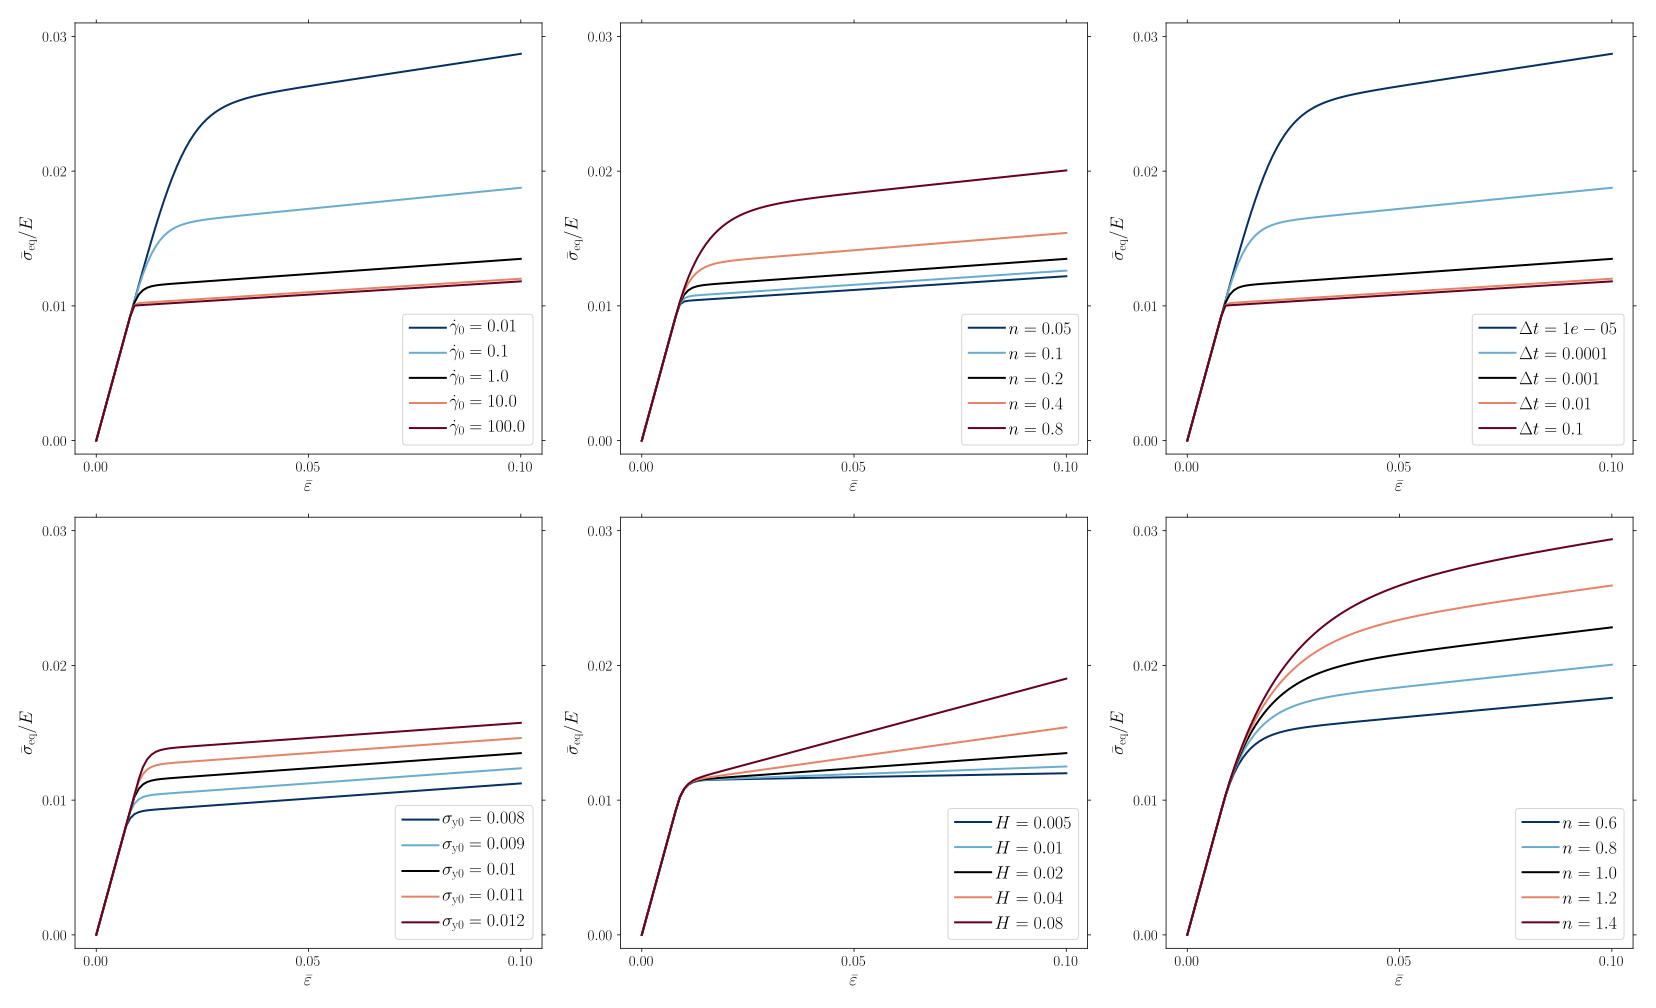
\includegraphics[width=1.\textwidth]{figures/parameters}
  \caption{Effect of different parameter variations.}
  \label{fig:parameter}
\end{figure}

\appendix
\vfill\newpage

\section{Nomenclature}
\label{sec:nomenclature}

\begin{itemize}
%
\item Dyadic tensor product
\begin{align}
  \mathbb{C} &= \bm{A} \otimes \bm{B} \\
  C_{ijkl}   &= A_{ij} \,      B_{kl}
\end{align}
%
\item Double tensor contraction
\begin{align}
  C &= \bm{A} : \bm{B} \\
    &= A_{ij} \, B_{ji}
\end{align}
%
\item Deviatoric projection tensor
%
\begin{equation}
  \mathbb{I}_\mathrm{d}
  = \mathbb{I}_\mathrm{s} - \tfrac{1}{3} \bm{I} \otimes \bm{I}
\end{equation}
%
\end{itemize}

\section{Stress measures}
\label{sec:ap:stress}

\begin{itemize}
%
\item Mean stress
%
\begin{equation}
\sigma_\mathrm{m}
= \tfrac{1}{3} \, \mathrm{tr} ( \bm{\sigma} )
= \tfrac{1}{3} \, \bm{\sigma} : \bm{I}
\end{equation}
%
\item Stress deviator
%
\begin{equation}
  \bm{\sigma}_\mathrm{d}
  = \bm{\sigma} - \sigma_\mathrm{m} \, \bm{I}
  = \mathbb{I}_\mathrm{d} : \bm{\sigma}
\end{equation}
%
\item Von Mises equivalent stress
\begin{align}
\sigma_\mathrm{eq}
= \sqrt{ \tfrac{3}{2} \, \bm{\sigma}_\mathrm{d} : \bm{\sigma}_\mathrm{d} }
= \sqrt{ 3 J_2(\bm{\sigma}) }
\end{align}
where the second-stress invariant
\begin{align}
J_2 = \tfrac{1}{2} \, || \, \bm{\sigma}_\mathrm{d} \, ||^2
    = \tfrac{1}{2} \, \bm{\sigma}_\mathrm{d} : \bm{\sigma}_\mathrm{d}
\end{align}
%
\end{itemize}

\section{Constitutive model in one-dimension}
\label{sec:1D}

\begin{enumerate}[(i)]
%
\item Elasto-plastic decomposition
\begin{equation}
  \varepsilon = \varepsilon_\mathrm{e} + \varepsilon_\mathrm{p}
\end{equation}
%
\item Linear elasticity
\begin{equation}
  \sigma = E \; \varepsilon_\mathrm{e}
\end{equation}
%
\item Yield function
\begin{equation}
  \Phi ( \sigma , \sigma_\mathrm{y} ) = | \sigma | - \sigma_\mathrm{y}
\end{equation}
Elastic domain
\begin{equation}
  \mathcal{E}
  = \big\{ \sigma \; \big| \; \Phi ( \sigma , \sigma_\mathrm{y} ) < 0 \big\}
\end{equation}
%
\item Plastic flow rule
\begin{equation}
  \dot{\varepsilon}_\mathrm{p} = \dot{\gamma} \; \mathrm{sign} ( \sigma )
\end{equation}
where
\begin{equation}
  \dot{\gamma}
  =
  \begin{cases}
    \displaystyle \dot{\gamma}_0
    \left[
      \left( \frac{| \sigma |}{\sigma_\mathrm{y}} \right)^{1/n} - 1
    \right] \qquad &
    \mathrm{if} \; \Phi ( \sigma , \sigma_\mathrm{y} ) \geq 0
    \\
    0 \qquad &
    \mathrm{if} \; \Phi ( \sigma , \sigma_\mathrm{y} ) <    0
  \end{cases}
\end{equation}
%
\item Hardening law
\begin{align}
  \sigma_\mathrm{y} &= \sigma_\mathrm{y0} + H \varepsilon_\mathrm{p}^m \\
  \dot{\varepsilon}_\mathrm{p} &= \dot{\gamma}
\end{align}
\end{enumerate}

\bibliography{library}

\end{document}


